\section{Preparazione del dataset}

\subsection{Dataset termico FLIR}
Il dataset termico utilizzato è fornito da Teledyne FLIR\cite{39}, un'azienda leader nel settore delle tecnologie di rilevamento termico e di imaging a infrarossi, ed è stato progettato per consentire agli sviluppatori di avviare l'addestramento di reti neurali convoluzionali, finalizzate alla creazione della prossima generazione di sistemi avanzati di assistenza alla guida (ADAS) e veicoli autonomi più sicuri ed efficienti.

Il dataset è composto da immagini catturate sia di giorno (60\%) che di notte (40\%) su strade e autostrade nell’area di Santa Barbara (California) da Novembre a Maggio, con condizioni meteorologiche sia limpide che nuvolose.

\vspace{0.5cm}

\begin{figure}[ht]
    \centering
    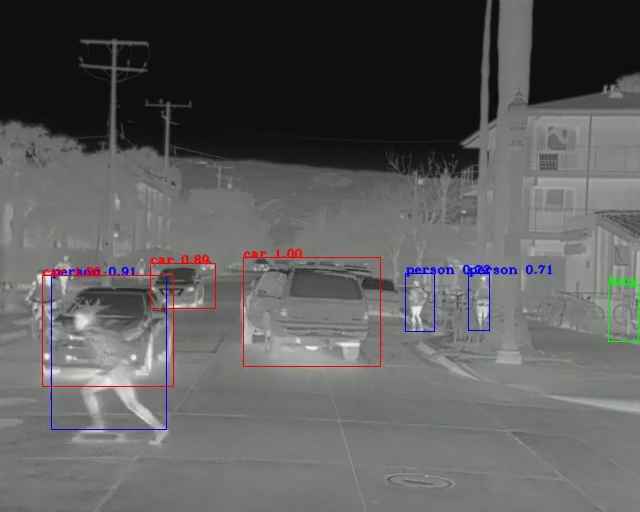
\includegraphics[width=0.8\textwidth]{files/capitoli/4-sperimentazione-risultati/assets/flir-example.png}
    \caption{\label{fig:flir-example}Immagine del dataset termico FLIR\cite{39}}
\end{figure}

\newpage

Le immagini sono state acquisite utilizzando una termocamera con le seguenti specifiche\cite{39}:
\begin{itemize}
    \item \textbf{Termocamera IR}: Tau2 640 x 512, 13 mm f/1,0 (HFOV 45°, VFOV 37°)
    \item \textbf{Telecamera FLIR BlackFly}: (BFS-U3-51S5C-C) 1280 x 1024, ottica megapixel Computar 4-8 mm f/1,4-16 (FOV impostato per Tau2)
\end{itemize}

\subsection{Estrazione e Formattazione dei subset}
Scaricando il dataset dalla apposita pagina di Teledyne FLIR\cite{39}, ci troviamo di fronte alle seguenti raccolte di immagini:

\begin{figure}[ht]
    \centering
    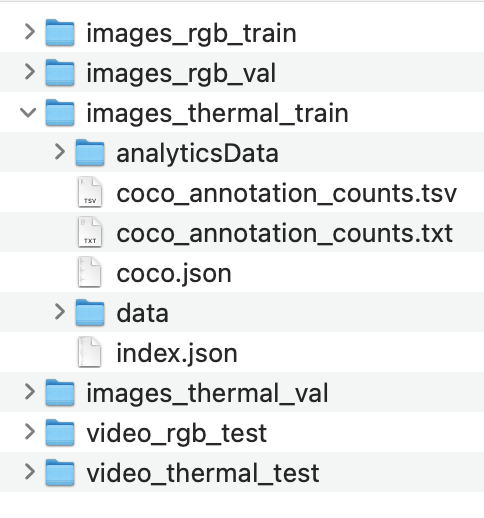
\includegraphics[width=0.35\textwidth]{files/capitoli/4-sperimentazione-risultati/assets/flir-adas.png}
    \caption{\label{fig:flir-adas}Contenuto di FLIR\textunderscore ADAS\textunderscore v2.zip}
\end{figure}

I dati di nostro interesse sono contenuti nelle cartelle relative alle immagini termiche ("thermal") per i 3 subset di train, val e test; le immagini termiche di ogni subset si trovano della cartella \texttt{data}, mentre le annotazioni nei file \texttt{coco.json} (formato MSCOCO) e \texttt{index.json} (formato di Conservator, un tool proprietario di Teledyne FLIR per il management dei dataset).

\newpage

Per addestrare i modelli YOLO, è necessario organizzare la cartella del dataset con la seguente struttura:

\begin{figure}[ht]
    \centering
    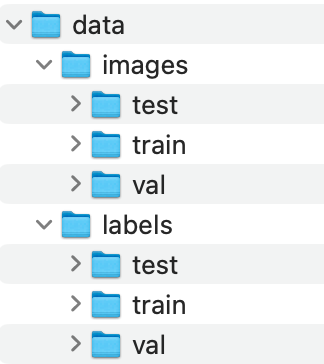
\includegraphics[width=0.23\textwidth]{files/capitoli/4-sperimentazione-risultati/assets/yolo-data-format.png}
    \caption{\label{fig:yolo-data-format}Struttura cartella dataset per i modelli YOLO}
\end{figure}

Tramite uno script Python sono quindi andato a copiare le immagini dei tre subset nelle relative cartelle in \texttt{data/images}, e successivamente sono andato a generare le annotazioni in formato YOLO di ciascuna immagine partendo da quelle presenti in \texttt{index.json}, inserendole in file di testo salvati in \texttt{data/labels}.

Perciò ciascuna immagine \texttt{(frameID).jpg} in \texttt{data/images/(subset)}, avrà il corrispettivo file di testo \texttt{(frameID).txt} in \texttt{data/labels/(subset)}, il quale contiene le relative annotazioni nel formato YOLO: ogni riga corrisponde ad una Bounding Box e contiene id della classe, coordinata X del centro, coordinata Y del centro, larghezza ed altezza.

\vspace{0.5cm}

\begin{figure}[ht]
    \centering
    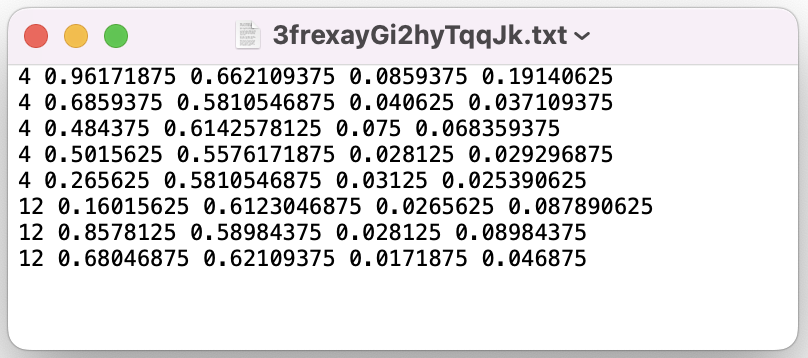
\includegraphics[width=0.7\textwidth]{files/capitoli/4-sperimentazione-risultati/assets/label-example.png}
    \caption{\label{fig:label-example}File contenente le annotazioni del frame "3frexayGi2hyTqqJk"}
\end{figure}


\subsection{Analisi delle classi}
Il dataset originario contiene le annotazioni relative a 20 classi di oggetti, segue l'analisi dettagliata del numero di annotazioni presenti nei 3 subset per ciascuna delle classi:

\begin{figure}[ht]
    \centering
    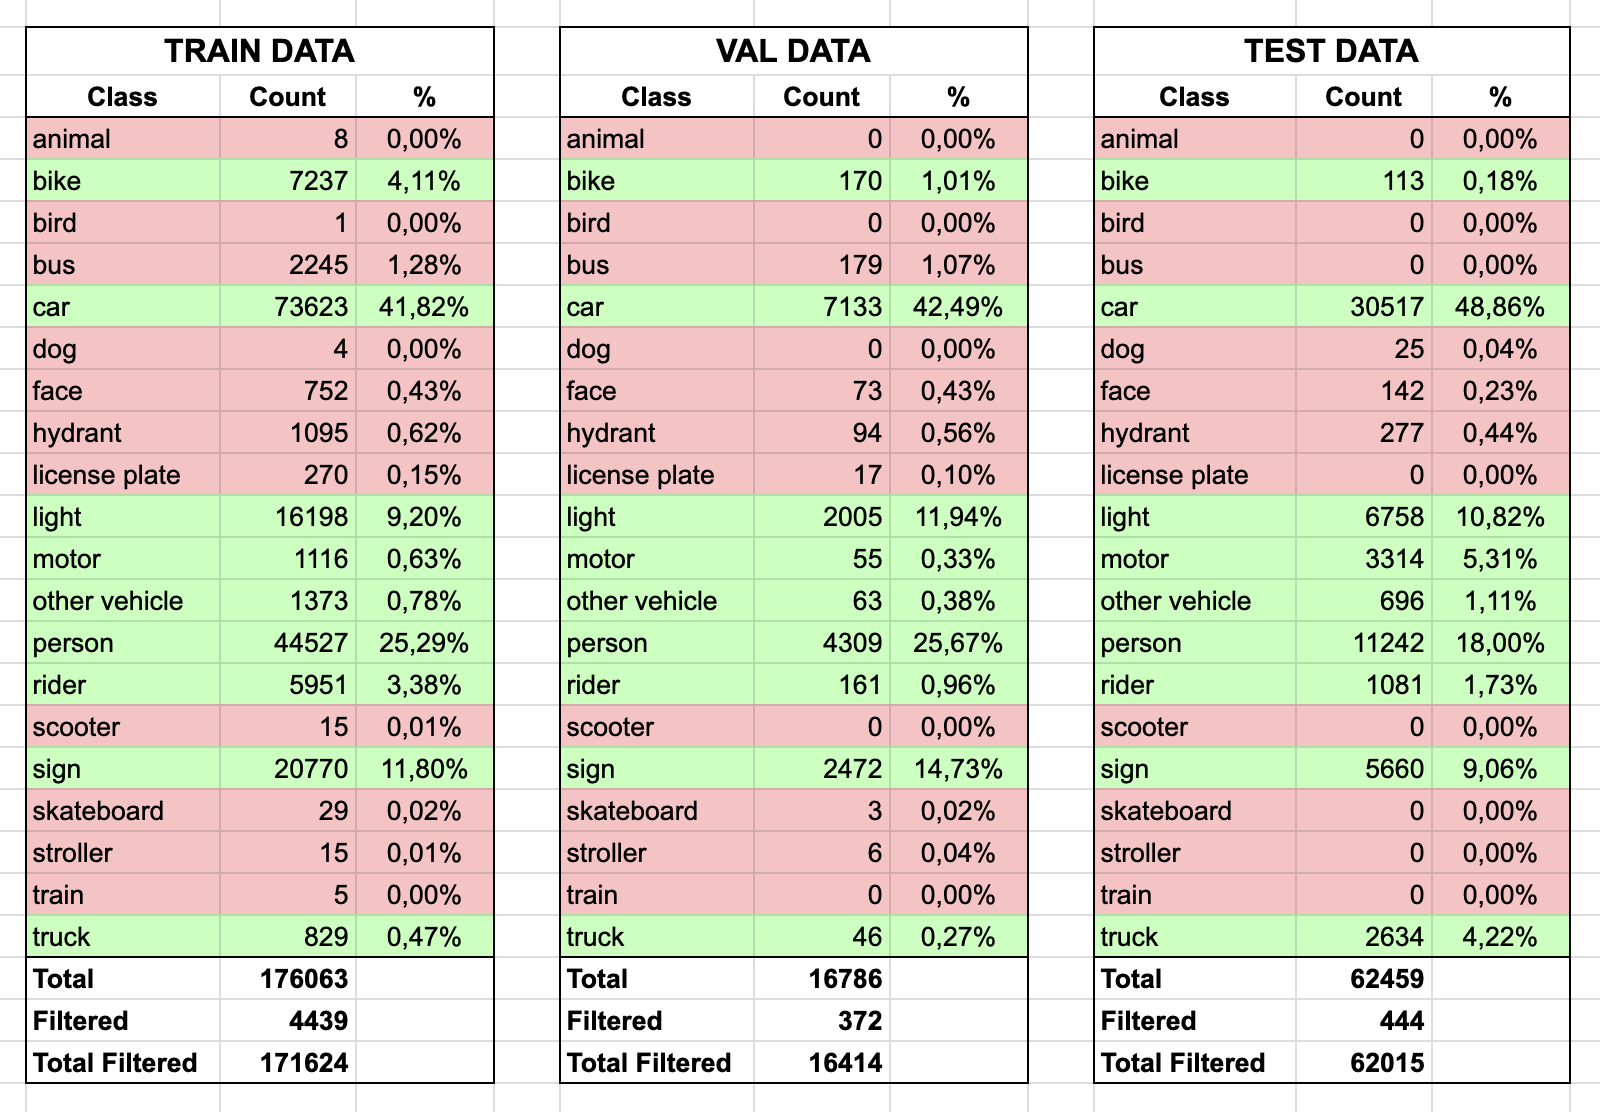
\includegraphics[width=1\textwidth]{files/capitoli/4-sperimentazione-risultati/assets/class-counts.png}
    \caption{\label{fig:class-counts}Analisi delle annotazioni per ciascuna classe}
\end{figure}

Possiamo notare che alcune classi sono sottorappresentate nelle annotazioni rispetto al totale, il che potrebbe compromettere l'efficacia dell'addestramento del modello e deteriorare le metriche di valutazione complessive.
Per questo motivo, ho deciso di filtrare le classi in questione dalle annotazioni del dataset (quelle evidenziate in rosso).

\newpage

\subsection{Nuovo dataset filtrato}
Ho quindi generato un nuovo dataset chiamato \texttt{filtered-data}, che contiene le stesse immagini dell'originale, ma con i file .txt delle annotazioni aggiornati. Le annotazioni sono state filtrate tramite uno script Python che ha scansionato le righe dei file di annotazione originali, rimuovendo quelle relative alle classi da escludere.

Così facendo, ho ottenuto il dataset su cui addestrare i modelli, suddiviso come segue:
\begin{itemize}
    \item \textbf{Train subset}: 10742 esempi
    \item \textbf{Val subset}: 1144 esempi
    \item \textbf{Test subset}: 3749 esempi
\end{itemize}

\newpage

